\chapter{Results}\label{results}
 
Based on the descriptions provided in the Methods section, the \verb|dSTRF| Python library was used for the implementation. The process involved training a convolutional neural network (CNN) to predict neuronal activity from auditory spectrograms, which was subsequently linearized to extract interpretable DSTRFs for individual pixels over time. 

\section{Overview} 
To provide an initial understanding of the neural activation across the auditory cortex and to establish a baseline for comparison with the DSTRF approach, traditional spectro-temporal receptive fields (STRFs) were computed. Figure \ref{fig:strf_m219_r25} illustrates the average activation over time of each pixel in the recording, derived from mouse 219, recording 25, trial 1, after fitting a ridge regression model. The color of each pixel signifies the mean STRF response of each neuron across both the temporal dimension, yielding a single aggregated value. From this visualization, two distinct regions were identified as exhibiting the strongest neuronal activity. Further insight into the temporal dynamics of the average STRF is provided by Figure \ref{fig:strf_temp_avg}. This figure, generated using the same underlying data as Figure \ref{fig:strf_m219_r25}, presents the STRF of each neuron summed exclusively across the spatial dimension. The output is a chronological sequence of frames, effectively creating a "video" that depicts the average STRF value at each discrete time point, providing a dynamic view of the neural response over time. This recording is also made available in the associated GitHub repository.

\begin{figure}[!htb]
	\centering
	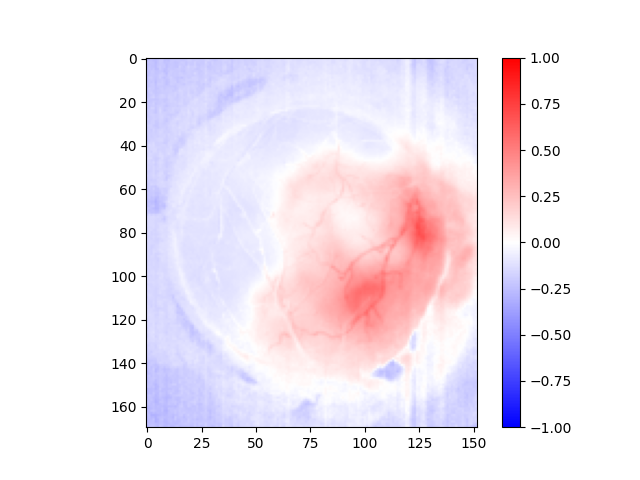
\includegraphics[scale=0.4]{m219_r25_t1/avg_strf}
	\caption{The figure shows the average activation over time of each pixel in the recording. The two axes represent the spatial coordinates of each pixel. Two regions can be identified as having the strongest activity.}
	\label{fig:strf_m219_r25}
\end{figure}

\begin{figure}[!htb]
	\centering
	\animategraphics[width=0.5\linewidth,controls]{30}{m219_r25_t1/video/image}{1}{31}
	\caption{This figure is generated using the same data as Figure \ref{fig:strf_m219_r25} but instead the STRF of each neuron is only summed accross the spatial dimension, resulting in a video where the average STRF value is shown for each moment $t$. The two axes represent the spatial coordinates of each pixel. This recording is also available in the github repository.}
	\label{fig:strf_temp_avg}
\end{figure}

Furthermore, Figure \ref{fig:50trials} quantifies the predictive performance of the DSTRF models by illustrating the average correlation scores per pixel between the actual recorded neural response and the response predicted by the DSTRF.

\begin{figure}[!htb]
	\begin{subfigure}{0.45\textwidth}
		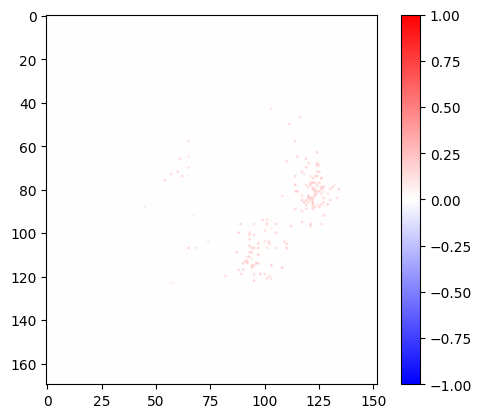
\includegraphics[width=\textwidth]{50_trials}
		\caption{This panel shows the correlation between the actual and predicted response. This network was trained on 40 trials, and 10 trials were used for testing. The scores (i.e correlations) were then averaged for each pixel and plotted here.}
		\label{subfig:50trials}
	\end{subfigure}
	\hfill
	\begin{subfigure}{0.45\textwidth}
		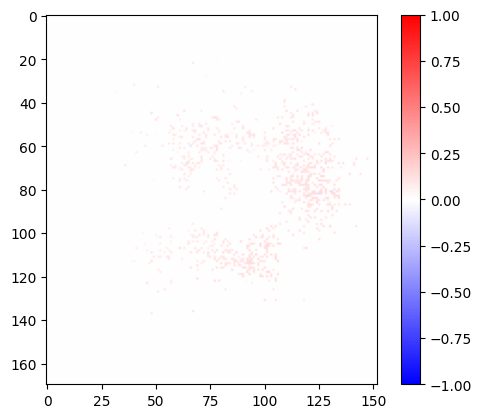
\includegraphics[width=\textwidth]{90_trials}
		\caption{The same procedure as in the left panel was applied here. In this case, 72 trials were used for training and 18 for testing. There are significantly more correlations visible in the figure, probably due to the increased amount of input data.}
		\label{subfig:90trials}
	\end{subfigure}
	\caption{The figure shows the average Pearson correlation scores per pixel between the actual response to the stimulus and the response predicted by the DSTRF. The two axes represent the spatial coordinates of each pixel. A comparison is made between models trained on varying amounts of data.}
	\label{fig:50trials}
\end{figure}

A comparative analysis was conducted across models trained on varying quantities of data. Figure \ref{subfig:50trials} displays correlations from a network trained on 40 trials, with 10 trials allocated for testing, where scores were averaged per pixel. Panel (b) follows the same procedure but with a larger dataset: 72 trials for training and 18 for testing. Notably, Figure \ref{subfig:90trials} exhibits significantly more visible correlations, suggesting that the increased amount of input data during training leads to more robust and higher predictive accuracy of the DSTRF model.

